%===============================================================================
% Autoři: Michal Bidlo, Bohuslav Křena, Jaroslav Dytrych, Petr Veigend a Adam Herout 2018
\chapter{Úvod}

Tento text slouží jako ukázkový obsah šablony a současně rekapituluje nejdůležitější informace z předpisů a poskytuje další užitečné informace, které budete potřebovat pro tvorbu technické zprávy ke svojí práci. Než se šablonou budete dále pracovat, je třeba vědět, jak ji správně použít. To je stručně uvedeno v~příloze \ref{jak}.

I když některým studentům pro napsání dobré diplomové práce (bakalářská práce je také diplomová -- dostává se za ni diplom) stačí znát a dodržovat oficiální formální požadavky uvedené ve směrnicích a typografické zásady, často je výhodné před započetím psaní zjistit, jaké jsou osvědčené postupy pro psaní odborného textu a jak si práci usnadnit. Někteří vedoucí svým studentům připravili popisy osvědčených postupů, které vedly k desítkám úspěšně obhájených prací. Výběr nejzajímavějších postupů, které měli autoři této šablony k~dispozici ve chvíli její tvorby, je v níže uvedených kapitolách. Má-li Váš vedoucí svoji stránku s doporučenými postupy, tyto kapitoly můžete vynechat a řídit se pokyny svého vedoucího. Pokud takovou stránku nemá, může být přečtení níže uvedeného textu vhodnou přípravou na konzultaci o plánované struktuře a náplni textu práce.

Diplomová práce je rozsáhlé dílo a tomu odpovídá i technická zpráva. Ne každý je schopen si sednout a jednoduše ji napsat. Je třeba vědět, kde začít a jak postupovat. Jedním z možných přístupů je začít psaním klíčových slov a abstraktu, abyste si ujasnili, co je v~práci nejdůležitější. O tom pojednává kapitola \ref{abstrakt}.

Po sepsání abstraktu se lze pustit do psaní samotného textu technické zprávy. Typicky si nejprve připravíme základní strukturu práce, kterou pak budeme plnit textem. Kapitola \ref{struktura} se zabývá základními informacemi a radami pro psaní odborného textu, které Vám pomohou vyhnout se začátečnickým chybám, a stanovením nadpisů kapitol a přibližných rozsahů jednotlivých částí práce. V závěru kapitoly je pak uveden přístup, kterým si lze psaní technické zprávy značně usnadnit.

Diplomové práce v oblasti informačních technologií mají určitou typickou strukturu. Po~úvodu bude následovat kapitola či kapitoly zabývající se shrnutím současného stavu, který bude v následujících kapitolách zhodnocen a bude navrženo řešení, které bude implementováno a otestováno. V závěru pak budou výsledky vyhodnoceny a bude navržen budoucí vývoj. I když se názvy a rozsahy kapitol v různých pracích liší, vždy tam lze najít kapitoly odpovídající této struktuře. Kapitola \ref{kapitoly} se zabývá obsahy typických kapitol, které se v diplomových pracích z oblasti IT vyskytují. Většina studentů ve svojí práci pravděpodobně využije pouze určitou podmnožinu popsaných kapitol, která je pro jejich práci relevantní. Uvedené popisy a rady mohou pomoci jak s~rozhodnutím, zda danou kapitolu uvést, tak i~s~vnitřní strukturou a samotným obsahem kapitoly.

Za závěrečnou kapitolou práce vždy následuje seznam použité literatury. Citacemi, které tento seznam tvoří, a odkazy na ně se zabývá kapitola \ref{citace}. Byť to tak nezkušený student nemusí vnímat, je seznam použité literatury a odkazy na něj pro práci zcela zásadní. Hodnocení práce s literaturou a citací tvoří jednu z důležitých částí posudku oponenta a bude-li chybět jediná položka, může to vést k hodnocení stupněm F, následnému disciplinárnímu řízení za plagiátorství a k vyloučení z nedokončeného studia. Nesprávná práce se zdroji může mít i další důsledky -- v roce 2018 stála křesla dva členy české vlády. Proto prosím citacím věnujte odpovídající pozornost. 

Po dokončení textu je nutné zjistit, jaké požadavky jsou kladeny na vysokoškolskou kvalifikační práci na FIT VUT v~Brně, a dořešit případné nedostatky. Formální požadavky jsou uvedeny ve směrnicích a na webových stránkách, které jsou zmíněny v kapitole \ref{formality}. Tato kapitola obsahuje i požadované rozsahy jednotlivých typů prací a další vybrané informace z~předpisů a doporučení. V závěru kapitoly je uveden přehled nejčastějších chyb, se kterými se oponenti setkávají a kterým byste se měli vyhnout. Hodnocení formální úpravy práce je pak další z důležitých součástí posudku oponenta.

Po odstranění formálních nedostatků lze práci odevzdat. Před odevzdáním práce si můžete projít kontrolní seznam (tzv. \uv{checklist}) uvedený v příloze \ref{checklist}. Samotné odevzdání listinné i elektronické verze práce je pak popsáno v kapitole \ref{odevzdani}.

V závěrečné kapitole \ref{zaver} je pak uvedeno shrnutí toho, co se lze přečtením tohoto textu dozvědět, a to nejdůležitější, na co je třeba myslet před odevzdáním práce.


\chapter{Testovanie softwaru}
\label{testing}
Testovanie softvéru je súbor procesov analyzujúcich softvér za účelom vyhodnotenia jeho vlastností a detekcie rozdieľov medzi aktuálnym a požadovaným stavom \cite{Standard}. Táto kapitola najskôr predstavuje základné úrovne a druhy testovania. Následne popisuje testovanie založené na dátach a s tým spojenú rozhodovaciu tabuľku. Rozoberá spôsoby tvorby a voľby dát rozhodovacej tabuľky. V závere predstavuje platfomu Testos.   

\bigskip
\section{Úrovne testovania}
Testy sú vytvárané na základe špecifikácií a požiadaviek, dizajnových artefaktov alebo zdrojového kódu. Rôzne úrovne testovania sprevádzajú rozdieľne vývojárske aktivity \cite{Ist}.
\subsection*{Jednotkové testovanie}
Jednotkové testovanie je zamerané na jednotky, predstavujúce najmenšie testovateľné komponenty testovaného systému. Zmyslom jednotkového testovania je validácia správania jednotky voči jej dizajnu. Zameriava sa na chyby na najnižšej úrovni. Testy vytvárajú samotný programátori počas vývoja.    
\subsection*{Integračné testovanie}
Integračné testovanie je cielené na korektnú komunikáciu medzi rozhraniami jednotiek, ktoré sú pre tento účel zlučované do podsystémov. Úlohou integračného testovania nie je nájdenie chýb v jednotlivých integrovaných jednotkách, ale overenie ich korektnej integrácií. Predpokladá sa, že tieto chyby boli eliminované pri jednotkovom testovaní. Odhaľuje chyby v rozhraniach a stavoch jednotiek. Pri väčšom množstve rozhraní je vhodné zvoliť špecifický prístup k integračným testom. Obvyklé stratégie sú zdola nahor, zhora dole, funkcionálna integrácia a veľký tresk \cite{Gst}. Obvykle ich tvoria vývojári alebo testeri v rámci tímu.
\subsection*{Systémové testovanie}
Systémové testovanie je zamerané na nájdenie chýb vo vlastnostiach plne integrovaného systému. Testovaný systém je tvorený komponentami, ktoré už úspešne prešli integračnými testami. Cieľom je detekcia nekonzistentností mezi týmito komponentami a systému ako ceľku voči špecifikácií požiadavkov. Systémové testovanie vykonáva oddelená skupina testerov mimo vývojový tím. 
\subsection*{Akceptačné testovanie}
Akceptačné testovanie je proces s účelom overenia softvéru voči počiatočným stanoveným požiadavkom zákazníka jeho aktuálnych potrebieb. Často sa na ich vytváraní podieľa expert na doménu, pre ktorý sa softvér vyvýja. Zvyčajne je vytvorený zákazníkom alebo koncovým užívateľom a overuje, že dané riešenie pre užívateľa funguje \cite{Ast}.  

\section{Dynamické testovanie}
\label{Dyn_t}
Existuje mnoho prístupov k testovaniu softvéru. Na najvyššej úrovni sa testovanie rozdeľuje na {\it statické} a {\it dynamické} \cite{Ist}. Techniky, ktoré analyzujú a skúmajú program bez nutnotsti jeho spusteniam za účelom verifikácie spadajú do skupiny statického testovania. Zahňuje posudzovanie dokumentov, kódu a jeho statickú analýzu (základná statická analýza zvyčajne prebieha na úrovni kompilátorov). Druhá skupina techník spadá do skupiny dynamického testovania, ktorá je zameraná na analýzu dynamického správania kôdu s cieľom jeho validácie. Prerekvizitou je úspešná kompilácia a spustenie kódu. Zahrňuje prácu so softvérom, kedy pre špecifické vstupy overuje a analyzuje správnosť výstupov.

 Dynamické testovanie môže byť ďalej rozdelené na {\it funkcionárne} a {\it nefukncionárne}. Kým funkcionárne testovanie adresuje splňenie požiadaviek, nefukcionárne je mierené na ostatné oblasti ako bezpečnosť, výkonnosť, použiteľnosť, správa pamäti a iné. Podľa znalosti kôdu sa delí na {\it black-box, white-box a grey-box} testovanie.
 
  Táto práca sa zamerieva na testovanie založené na dátach, ktoré vychádza z funkcionálneho black-box testovania, ale výsledný nástroj môže byť prínosný aj pre iné prístupy.

       
\subsection*{Black-box testovanie}
{\it Black-box testovanie} (tiež známe ako {\it testovanie založené na dátach}) zoskupuje techniky tvorby testovacích prípadov na základe špecifikácií podľa analýzi popisu softvéru bez znalosti jeho vnútornej štruktúry  \cite{Ast}. Ich hlavným zameraním je odhalenie okoľností, pri ktorých sa systém správa odlišne od špecifikácií.  Testovacie dáta závisia na popise očakávaní od testovaného softvéru napríklad vo forme manuálu či popisu procesu.

Black-box testovanie môže byť využité na všetkých úrovniach testovania. Pre nižšie úrovne jednotkového a integračného testovania sa dá využiť ako počiatočný bod pre tvorbu testov na základe dizajnu alebo aj požiadaviek. Veľmi užitočné sú na vyžších úrovniach, teda systémová a akceptačná, kde sú testy založené na požiadavkách  \cite{Gst}.

\subsection*{White-box testovanie}
Techniky white-box testovania vytvárajú testovacie prípady podľa vnútornej štruktúry komponenty alebo systému. Hlavný dôraz kladú na vetvy, jednotlivé podmienky a výrazy tradične v zdrojovom kóde. Primárne sa využívajú v jednotkovom a integračnom testovaní. Všetky testovacie techniky tohoto druhu od testera vyžadujú znalosť danej štruktúry, teda programovacieho jazyka \cite{Gst}.    
\subsection*{Grey-box testovanie}
Mezi white-box a black-box testovaním je mnoho úrovní grey-box testovania ktoré predstavuje ich kombináciu. Testovacie prípady sú tvorené so znalosťou architektúry, algoritmov, vnútorných stavov alebo iného vysoko úrovňového popisu správania.
\section{Testovanie založené na dátach}
Jednoduché automatizované testovacie skripty obsahujú pevne dané testovacie dáta. Zmena týchto dát obvykle vyžaduje zmenu v zdrojovom kóde skriptu, čo môže viesť k viacerím komplikáciám. Ak je test neprehľadný, dlhý alebo neštrukturovaný, jednoduchá zmena v dátach je náročná aj pre skúsených expertov. Rovnako vzniká riziko zavedenia novej chyby. Pri tvorbe nových testov, líšiacich sa len v testovacích dátach, často dochádza k skopírovaniu kódu a následnej modifikácii dát. Pritom nastáva duplicita kódu a testovacie prípady sú ťažko udržateľné. 

Pri veľkých testovacích sadách sú pre spomenuté problémy skripty s pevne danými dátami len ťažko použiteľné. {\it Testovanie založené na dátach (Data-driven testing)} je metodológia , v ktorej sa opakovane vykonávajú rovnaké kroky skriptu s použitím externých dátových zdrojov. Takéto dáta musia byť ľahko editovateľné aj testerom bez znalosti zdrojového kódu. Umožňuje mu tým sústrediť sa len na tvorbu testovacích prípadov. Výhody metodológie sú zreteľné najmä pri aplikáciách s častými zmenami funkcionality. Hlavné výhody sú nasledovné \cite{Sttc}:
\begin{itemize}
	\item{Testy založené na dátach dosahujú vysoké pokrytie kódu testovacími prípadmi a zároveň minimalizujú množstvo kódu, ktoré je potrebné napísať a udržiavať}
	\item{Uľahčuje vytváranie a spúšťanie veľkého množstva testovacích podmienok}
	\item{Testovacie dáta môžu byť navrhnuté a vytvorené pred tým, ako je aplikácia pripravená na testovanie}
	\item{Rozhodovacie dátové tabuľky môžu byť použité pri manuálnom testovaní}
\end{itemize}
\begin{figure*}[h]\centering
	\centering
	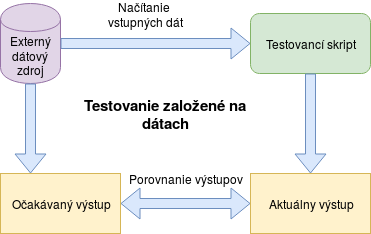
\includegraphics[width=3.5in,height=2.2in]{obrazky-figures/Data-driven_testing.png}\\[1pt]
	\caption{Diagram záladnej štruktúry testovania založeného na dátach .}
	\label{Tdd_img}
\end{figure*}
\section{Editácia a uloženie testovacích dát}
Využívané testovacie dáta sa obecne skladajú z kombinácie vstupných a očakávaných výstupných dát. Daný typ dát sa najlepšie popisuje formou {\it rozhodovacích tabuliek}. Rozhodovacia tabuľka v najjednoduchšej forme poskytuje vstupy ako aj očakávané výstupy na jednom riadku. Pri tvorbe tabuľky je dôležitá správna identifikácia všetkých vstupných dát a ich rozdelenie do {\it domén}. Výber konkrétnych hodnôt záleží od zvoleného prístupu \cite{Ast}. Najčastejšie sa využívajú nasledovné prístupy:
\begin{itemize}
	\item{ \textit{Testy pokrývajúce logiku}. Testovacie prípady spoločne dosahujú všetky definované výstupy a rovnako zaručujú vykonanie všetkých častí kódu minimálne raz.}
	\item{ \textit{Rozdelenie na ekvivalenčné triedy} \ref{ekv_tr}. 
		Vstupy sa rozdeľujú  do tried za účelom redukcie počtu testov. Predpokladá sa, že test na jednom prvku triedy reprezentuje všetky ostatné. }
	\item{ \textit{Analýza hraničných hodnôt}. 
		Prístup využíva ekvivalenčné triedy, jednotlivých reprezentantov ale nevolí náhodne. Keďže najčastejšie chyby sa vyskytujú pri hraničných hodnotách, konkrétne hodnoty volí z hraničných oblastí. Zohľadňuje pritom vstupné aj výstupné dáta.}
	\item{ \textit{Grafy príčin a dôsledkov (angl. Cause-Effect Graph)} \ref{ceg}. 
		Vytvárajú logickú grafovú reprezentáciu mezi požiadavkami a výsledkami testov. Pomáhajú pri výbere účelných a úplných testov.}
\end{itemize}


Vzhľadom k charakteru dát sa k ich editácii prirodzene ponúka využitie tabuľkových procesorov (anglicky{\it spreadsheet}). Prácu s danými programmi obvykle zvládajú testeri ako aj ľudia z oblasti biznisu, čo uľahčuje ich rýchle zapojenie. Dané programy sa často používajú aj na jednoduchý manažment testov pre manuálne testovanie. V tomto prípade sa dáta môžu zdieľať s automatizovanými testami a predchádať tak ich zbytočnej redundancii. Príklad tabuľky je uvedený na obrázku \ref{Domtab_img}. 
\begin{figure*}[h]\centering
	\centering
	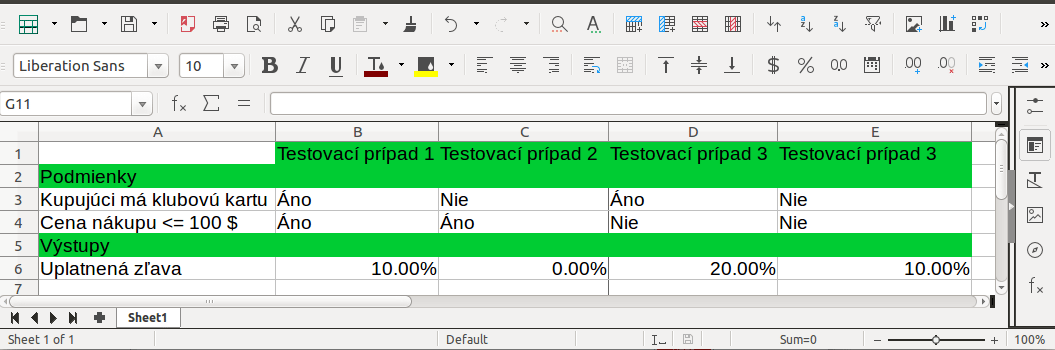
\includegraphics[width=6.0in,height=2.2in]{obrazky-figures/decision_table.png}\\[1pt]
	\caption{Príklad rozhodovacej tabuľky pre uplatnenie zľavy vytvorenej v tabuľkovom editore.}
	\label{Domtab_img}
\end{figure*}

Formáty uloženia tabuliek spadajú do viacerých kategórií. Prostý databázový soubor (anglicky flat file database) je jednoduchá databáza (väčšinou tabulka) uložená v textovom súbore ve forme prostého textu. Obvykle používané formáty sú napríklad hodnoty oddelené čiarkami (CSV), hodnoty oddelené tabulátormi (CSV, TXT) alebo iný špecifický formát (variácie XLS). Rovnako sú stále viac využívané štrukturované formáty ako XML a Json. Súčasné programovacie jazyky majú knižnice pre ich načítanie a spracovanie, čo výrazne uľahčuje ich využitie. Prosté dabázové súbory môžu mať problémy pri výraznom rozšírovaní. Rovnako je v nich neprehľadné uchovávanie rôznych konfigurácií a verzií. 

Pre veľké množstvo testovacích dát je vhodné využitie relačnej databázy. Umožňuje editáciu prostredníctvom skriptov ako aj pomocou grafických editorov.       
 

\section{Ekvivalenčné triedy a kritéria pokrytia}
\label{ekv_tr}
Zmyslom tvorby testovacích prípadov je nájdenie vstupov, ktoré najlepšie pokrývajú zvolené kritérium pokrytia. V závislosti od zložitosti testovaného softvéru môže byť množstvo možných vstupov  potenciálne nekonečné, preto je zvolenie vhodnej množiny testovacích dát náročné \cite{Gst}.
\subsection*{Rozdelenie vstupných domén na ekvivalenčné triedy}
Kľúčová je správna identifikácia vstupných domén. {\it Vstupná doména} testovaného systému je definovaná množinou všetkých vstupných hodnôt, ktoré nadobúda. V závislosti na testovacej úrovni a testovaného artefaktu sú to obvykle parametre metód, statické a globálne premenné, objekty reprezentujúce stav systému, uživateľské vstupy a argumenty programu \cite{Ist}. Vstupná doména je následne rozdelená na {\it ekvivalenčné triedy} (označované aj ako bloky). Pojem ekvivalencie sa vzťahuje k predpokladu, že všetky hodnoty v jednej tiede obsahujú z pohľadu testovania rovnako užitočné hodnoty. Každý prvok patrí práve do jednej tiedy a jediný prvok z ekvivalenčnej množiny reprezentuje všetky prvky. Keď overíme testovací prípad pre jeden prvok, predpokladáme, že sme overili všetky prvky z danej množiny. 

Pri rozpade domény \(D\) podľa rozdelenia \(q\) vznikajú vzájomne disjunktné ekvivalenčné triedy (bloky) \(B_{q}\)  definované nasledovne:

\begin{center}
	\(b_{i} \cap b_{j} = \emptyset , i \neq j ; b_{i} , b_{j} \in B_{q}\)
\end{center}


a spolu pokrývajú doménu \(D\)

\begin{center}
	\( \underset{b \in B_{q}}  \bigcup b = D\)
\end{center}
%\begin{figure*}[h]\centering
%	\centering
%	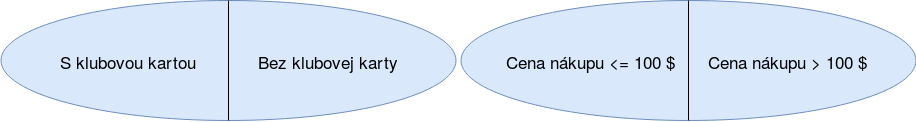
\includegraphics[width=6.5in,height=1.0in]{obrazky-figures/Domeny_dia.png}\\[1pt]
%	\caption{Rozpad domén z tabuľky \ref{Domtab_img} na ekvivalenčné triedy}
%	\label{Domdia_img}
%\end{figure*}
\begin{figure*}[h]\centering
	\centering
	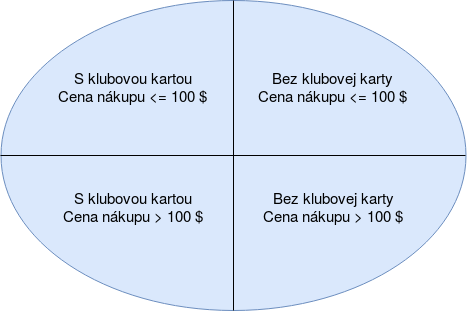
\includegraphics[width=3.5in,height=2.2in]{obrazky-figures/Domeny_all_dia.png}\\[1pt]
	\caption{Rozpad domén z tabuľky \ref{Domtab_img} na ekvivalenčné triedy}
	\label{Domdia_img}
\end{figure*}
\subsection*{Kritéria pokrytia}
Po identifikácií vstupných blokov je ďalší krok vytvorenie konkrétnej testovacej sady. Efektívne testovanie množstva blokov vyžaduje vhodný výber ich kombinácií. Stratégie zvolenia kombinácií sú dané konkrétnym krytériom pokrytia. \textit{Kritérium pokrytia (angl. Coverage criterion)} je pravidlo alebo predpis pre systematické generovanie požiadavkov na test. \textit{Pokrytie (angl. coverage)} je miera udávajúca, ako veľmi daná testovacia sada skúma testovaný systém. Obvykle sa udáva v percentách a viaže sa na konkrétne kritérium \cite{Ist}.     
 \begin{itemize}
 	\item{ \textit{Kritérium pokrytia všetkých kombinácií(angl. All Combinations Coverage)}. Kritérium vyžaduje pokrytie všetkých kombinácií blokov zo všetkých domén. Testovacie prípady spoločne dosahujú všetky definované výstupy a rovnako zaručujú vykonanie všetkých častí kódu minimálne raz. Reálne sa dá použiť len pri minimálnom množstve blokov.
 		}
 	\item{ \textit{Kritérium pokrytia všetkých párov blokov (angl.  Pair-Wise Coverage)}. Kritérium vyžaduje kombináciu každého bloku každej domény s každým blokom každej inej domény, teda všetkých dvojíc blokov z rôznych domén. Generalizáciou kritéria je \textit{Kritérium pokrytia všetkých n-tíc blokov (angl. T-Wise Coverage).}  
 	}
 	\item{ \textit{Kritérium pokrytia bázových blokov (angl. Base Choice Coverage)}. Pre každú doménu je zvolený bázový blok,  zvyčajne ide o najčajstejší alebo najdôležitejší blok. Kritérium vyžaduje kombinácie všetkých bázových blokov každej domény a pokrytie každého nebázového bloku. Vhodne zvolené kombinácie bázových blokov výrazne redukujú celkový počet testovacích prípadov. Vyžší stupeň predstavuje \textit{Kritérium pokrytia viacerých bázových blokov (angl. Multiple Base Choices Coverage)} 
 	} 	
 	\item{ \textit{Kritérium pokrytia každého bloku (angl. Each Choice Coverage)}. Kritérium vyžaduje pokrytie každého bloku pre každú domén. Minimálny počet testov sa rovná počtu blokov. Kritérium nieje veľmi efektívne a samotnú voľbu testovacích prípadov necháva na testerovi. Nevyžaduje žiadnu kombináciu hodnôt a preto je považované za slabé.
 	}
 \end{itemize}


\section{Grafy príčin a dôsledkov}
\label{ceg}
Slabinou predstaveného prístupu založeného na rozklade na ekvivalenčné triedy je absencia kombinácií vstupov. Riešenie ponúkajú spomenuté kritéria pokrytia, ale počet kombinácií vstupných dát je napriek tomu obvykle príliš vysoký. \textit{Graf príčin a dôsledkov (angl. Cause-Effect Graphing, CEG)} je grafický spôsob znázornenia prepojenia vstupov \textit{(príčiny, angl. causes)} s nimi asociovanými výstupmi \textit{(dôsledky, angl. effects)}. Graf je formálne vyjadrenie boolovských požiadavkov a umožňuje systematický spôsob výberu podmnožiny testovacích prípadov. 
Výhody prístupu sú nasledovné:
 \begin{itemize}
 	\item{ Redukcia počtu kombinácií vstupov
 	}
 	\item{ Odhalenie nejasností a nekompletnosti špecifikácie
 	}
 	\item{ Zrozumiteľný a jasne čitateľný formát
 	}
 	\item{ Zlepšenie celkového chápania systému a jeho dôležitých faktorov 
 	} 	
 	\item{ Pomoc pri hľadaní zdroja konkrétnej príčiny a dôsledkov  
 	} 	
 \end{itemize}
 Pre tvorbu testovacích prípadov je použitý nasledovný proces \cite{Ast}:
 \begin{enumerate}
 	\item{ \textit{Rozdelenie požiadavkov do skupín primeranej veľkosti.} Veľké množstvo požiadavkov by vyústilo do príliš veľký grafu, ktorý sa stane nepoužiteľným. 
 	}
 	\item{ \textit{Identifikácia príčin a dôsledkov.} Príčina je priamo vstupná podmienka alebo jej ekvivalenčná trieda. Dôsledok je výstupná podmienka alebo zmena v systéme.  
 	} 	
 	\item{ \textit{Analýza významu požiadavkov a vytvorenie grafu príčin a dôsledkov.} 
 	} 
 	\item{ \textit{Identifikácia obmedzení medzi príčinami a dôsledkami.} 
 	} 
 	\item{ \textit{Konvertovanie grafu do rozhodovacej tabuľky.} 
 	}  	
 	\item{ \textit{Každý stĺpec v tabuľke reprezentuje testovací prípad.}
 	}  		
 \end{enumerate}

\subsection*{Notácia grafu}
Základná notácia grafu je ukázaná na obrázku \ref{ceg_img}. Každý uzol môže nadobúdať hodnoty 0 a 1 reprezentujúce absenciu a prítomnosť stavu. Celkovo syntax pokrýva štyri prípady \cite{Ast}: 
 \begin{itemize}
 	\item{Funkcia \textit{identity}: ak \(a = 1\) tak \(b = 1\), inak \(b = 0\) 
 	}
 	\item{Funkcia \textit{NOT}: ak \(a = 1\) tak \(b = 0\), inak \(b = 1\) 
 	}
 	\item{Funkcia \textit{OR}: ak \(a\), \(b\) alebo \(c\) je rovné \(1\), tak \(d = 1\) 
 	} 		
 	\item{Funkcia \textit{AND}: ak \(a = 1\) a súčastne \(b = 1\), tak \(c = 1\), inak \(c = 0\)  
 	} 
 \end{itemize}
\begin{figure*}[h]\centering
	\centering
	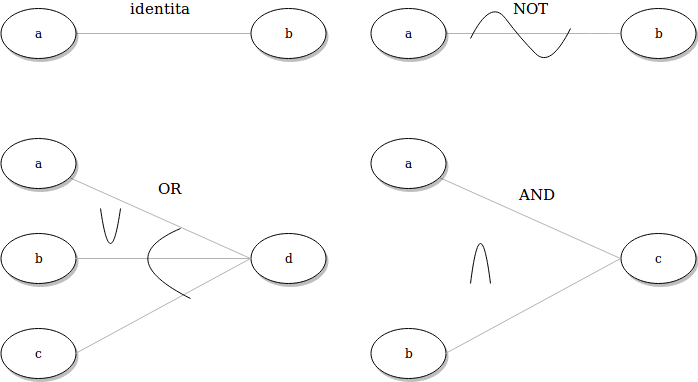
\includegraphics[width=4.5in,height=2.2in]{obrazky-figures/ceg.png}\\[1pt]
	\caption{Základné symboli CEG grafu \cite{Ast}.}
	\label{ceg_img}
\end{figure*}
Niektoré kombinácie medzi príčinami a dôsledkami sú neuskutočniteľné. Grafová reprezentácia na obrázku \ref{ceg_cons_img} preto umožňuje obmedzenia popísať nasledovne \cite{Ast}:
 \begin{itemize}
 	\item{Obmedzenie \textit{E}: Najviac jeden z uzlov \(a\) a \(b\) je súčasne rovný \(1\) 
 	}
 	\item{Obmedzenie \textit{I}: Aspoň jeden z uzlov \(a\), \(b\) a \(c\) je vždy rovný \(1\) 
 	}
 	\item{Obmedzenie \textit{O}: Práve jeden z uzlov \(a\) a \(b\) je  rovný \(1\) 
 	} 		
 	\item{Obmedzenie \textit{R}: Aby \(a\) moholo byť \(1\), \(b\) musí byť \(1\) 
 	}
 \end{itemize}    
 \begin{figure*}[h]\centering
 	\centering
 	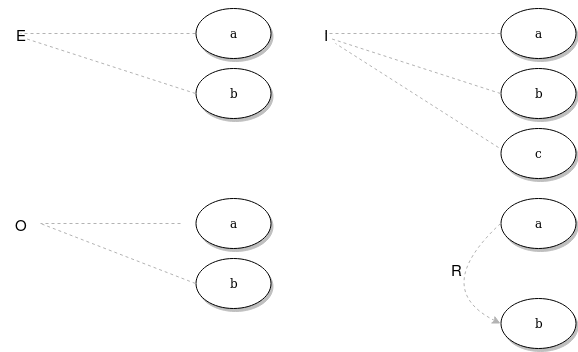
\includegraphics[width=4.5in,height=2.2in]{obrazky-figures/ceg_cons.png}\\[1pt]
 	\caption{Základné symboli CEG grafu \cite{Ast}.}
 	\label{ceg_cons_img}
 \end{figure*} 
      
\section{Testos}
Platforma \textit{Testos} (Test Tool Set) \cite{Testos} je projekt, ktorého hlavný cieľ je vytvorenie ucelenej sady nástrojov podporujúce automatizované testovanie softvéru. Platforma sa sústreďuje na všetky úrovňe testovania a podľa zamerania je rozdelená na oblasti:
\begin{itemize}
 	\item{Testovanie grafického uživateľského rozhrania \textit{(GUI)}
 	}
 	\item{Testovanie založené na modeloch \textit{(Model-based)}
 	}
 	\item{Testovanie založené na požiadavkach \textit{(Requirement-based)}
 	} 	
 	\item{Testovanie založené na dátach \textit{(Data-based)}
 	} 	
 	\item{Dynamická analýza \textit{(Execution-based)}
 	} 	
\end{itemize}  
Oblasť testovania založeného na dátach aktuálne obsahuje nástroje pre generovanie testovacích dát pre databázy (náhodné dáta, kombinácie dát a ich mutácie), detektory databázovej štruktúry a detektory štrukturovaných dát. Nástroj vytvorený v tejto práci patrí do rovnakej oblasti, v rámci nej priamo komunikuje a využíva ostatné nástroje Testos.

 \begin{figure*}[h]\centering
 	\centering
 	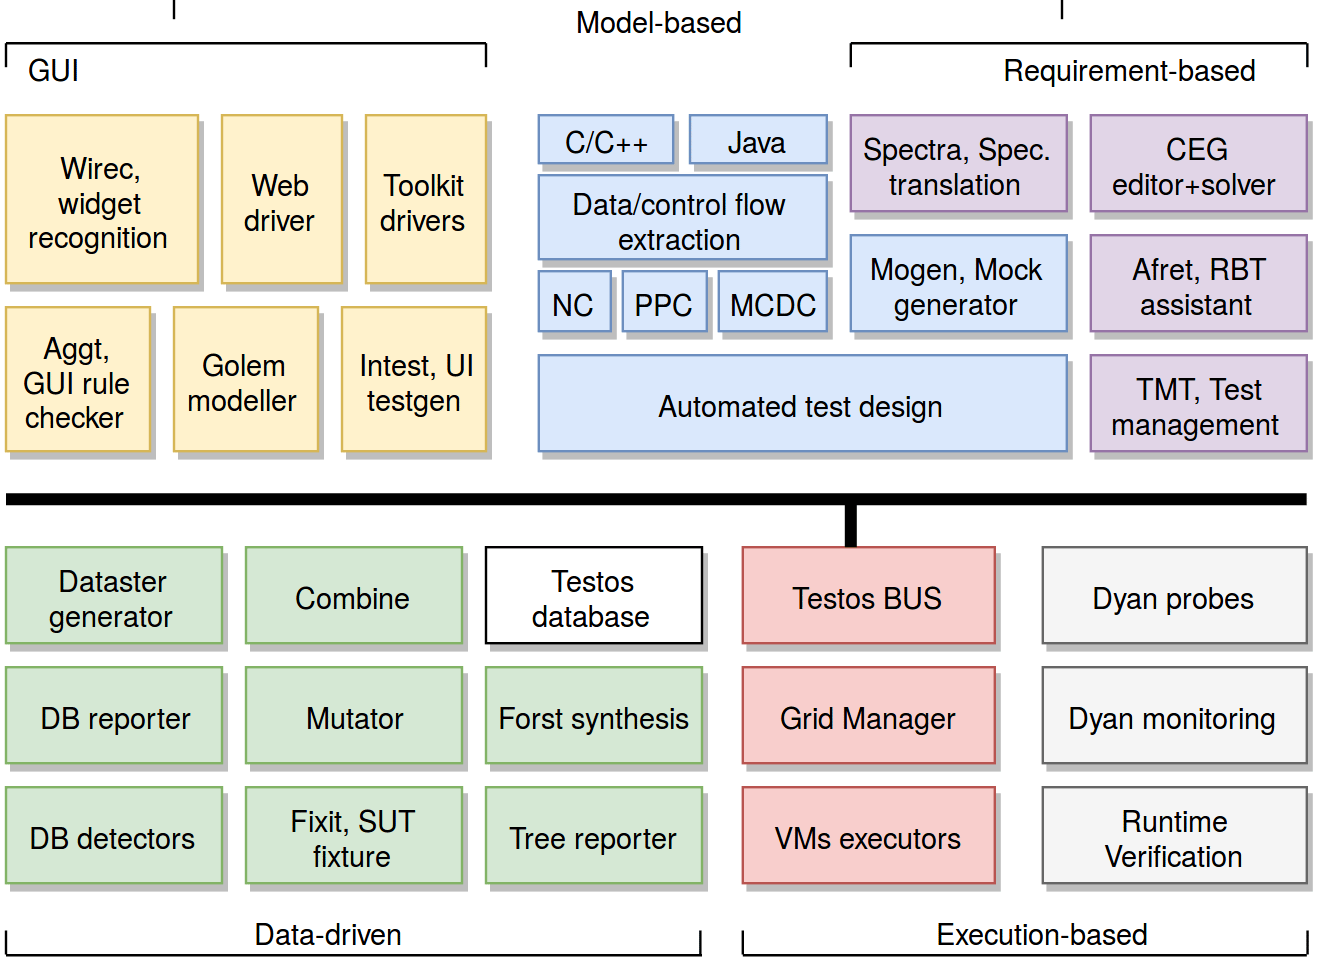
\includegraphics[width=6.0in,height=4.2in]{obrazky-figures/testos.png}\\[1pt]
 	\caption{Platforma Testos \cite{Testos}.}
 	\label{testos_img}
 \end{figure*} 


\chapter{Štrukturované dáta} 
\label{struktury}

Disponovanie vhodnými \textit{testovacími dátami} je pre proces testovania rovnako dôležité ako konkrétne prípady. S narastajúcou veľkosťou a komplexnosťou systémov je získanie takýchto dát stále obtiažnejšie. V tejto kapitole je najskôj uvedená obecná charakteristika štrukturovaných dát a spôsob ich grafovej reprezentácie. Následne sa venuje metódam ich porovnania z pohľadu štruktúry a sémantiky, pričom rozoberá problematiku klasterizácie. Nakoniec poskytne prehľad používaných formátov a existujúcich riešení získania testovacích dát.

\section{Grafová reprezentácia}
\section{Porovnávanie dát}
\section{Klasterizácia}
\section{Prehľad používaných formátov}
\section{Problém generovania}
\section{Existujúce generátory}





\chapter{Závěr}
\label{zaver}

V tomto textu bylo uvedeno, jak začít s tvorbou bakalářské či diplomové práce, napsat abstrakt, připravit základní strukturu práce a co uvést do jednotlivých kapitol. Při tom bylo vysvětleno, že bakalářská práce je také diplomová a je třeba k ní přistupovat stejně zodpovědným způsobem. Následně byla věnována pozornost bibliografickým citacím a formální stránce práce. V předposlední kapitole jsou uvedeny důležité informace k odevzdání v listinné i v elektronické podobě.

Je třeba zdůraznit, že diplomová práce je unikátním individuálním dílem, které vzniká pod vedením zkušeného odborníka. Ať už je v této šabloně uvedeno cokoliv, závazné jsou pouze oficiální pokyny na stránkách fakulty. Pro konkrétní diplomovou práci je potřeba vždy zvažovat, co je z výše uvedeného textu relevantní a co nikoliv a řídit se především pokyny vedoucího, který rozumí dané problematice a je tak schopen poskytnout ty nejlepší rady, co lze k práci dostat.

I přes velkou snahu nikdy není možné do šablony zahrnout všechny prvky, co budou při tvorbě práce potřeba, a zaručit, že po doplnění textu, obrázků, literatury apod. bude vše v~pořádku pro všechny možné diplomové práce. Bude-li někde delší text, než se předpokládalo, a zalomí-li se na dva řádky, bude-li v literatuře položka, se kterou nebyl otestován využitý styl, a v dalších případech může být výsledek neuspokojivý a může být potřeba do~šablony zasáhnout a chybu, která se projevuje třeba jen pro jednu práci ze sta, opravit. Výsledné PDF a následně i vytištěnou papírovou verzi je tedy vždy nutné pečlivě zkontrolovat a~nespoléhat se na to, že \uv{tohle přece generuje šablona, tak to musí být správně}. Najdete-li v šabloně nějaké chyby nebo budete-li mít návrhy na její vylepěšení, napište prosím na e-mail sablona@fit.vutbr.cz a pomozte nám s jejím vylepšováním. Veškeré připomínky a návrhy jsou vítány.

S kontrolou výsledku může výrazně pomoci vedoucí práce. Nelze však předpokládat, že vedoucí poslední noc před odevzdáním bude sedět v práci připraven na kontrolu desítek stran textu. Proto je nutné mít vše připravené v předstihu a konzultovat průběžně. Kritický pohled vedoucího pak umožní dosažení kvalitního výsledku a aktivita, kterou uvidí, přispěje k pozitivnímu hodnocení práce z jeho strany.

Na závěr bych jménem autorů této šablony popřál všem, kteří právě vytvářejí svoje diplomové práce nebo se k jejich tvorbě připravují, úspěšné dokončení a obhájení práce.






%===============================================================================
